\appendix
\chapter{Individual Constructions}

We diagram lethal set constructions for single grids. The initial infection $A$ is colored red, and all other cells are labeled with the time $t$ that they are first infected. 

\section{Perfect constructions}

% (3,3,1)
\begin{con}
\label{con:3x3x1}
The grid $G(3,3,1)$ is perfect.
\end{con}

\begin{proof}
See Figure \ref{fig:3x3x1_numbered_heatmap}.
\end{proof}

\begin{figure}[H]
\centering
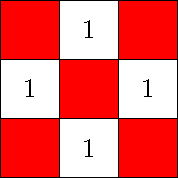
\includegraphics[width=0.14\textwidth]{figures/A/3x3x1_numbered_heatmap.pdf}
\caption{Time-steps of infection from a perfect lethal set on $G(3,3,1)$.}
\label{fig:3x3x1_numbered_heatmap}
\end{figure}

% (2,2,2)
%\begin{con}
%\label{con:2x2x2}
%The grid $(2,2,2)$ is perfect.
%\end{con}

%\begin{proof}
%See Figure \ref{fig:2x2x2_numbered_heatmap}.
%\end{proof}

%\begin{figure}[H]
%\centering
%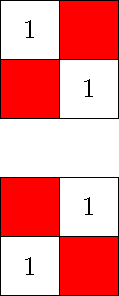
\includegraphics[width=0.2\textwidth]{figures/A/2x2x2_numbered_heatmap.pdf}
%\caption{}
%\label{fig:2x2x2_numbered_heatmap}
%\end{figure}

% (5, 2, 2)
\begin{con}
\label{con:5x2x2}
The grid $G(5,2,2)$ is perfect.
\end{con}

\begin{proof}
See Figure \ref{fig:2x5x2_numbered_heatmap}.
\end{proof}

\begin{figure}[H]
\centering
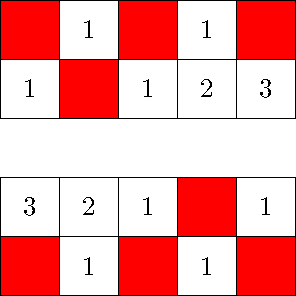
\includegraphics[width=0.24\textwidth]{figures/7/2x5x2_numbered_heatmap.pdf}
\caption{Time-steps of infection from a perfect lethal set on $G(5,2,2)$.}
\label{fig:2x5x2_numbered_heatmap}
\end{figure} 

\newpage

% (5,5,2)
\begin{con}
\label{con:5x5x2}
The grid $G(5,5,2)$ is perfect.
\end{con}

\begin{proof}
See Figure \ref{fig:5x5x2_numbered_heatmap}.
\end{proof}

\begin{figure}[H]
\centering
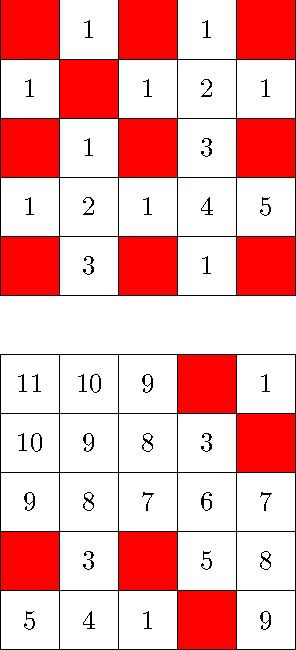
\includegraphics[width=0.2\textwidth]{figures/A/5x5x2_numbered_heatmap.pdf}
\caption{Time-steps of infection from a perfect lethal set on $G(5,5,2)$.}
\label{fig:5x5x2_numbered_heatmap}
\end{figure}

% (3,3,3)
%\begin{con}
%\label{con:3x3x3}
%The grid $(3,3,3)$ is perfect.
%\end{con}

%\begin{proof}
%See Figure \ref{fig:3x3x3_numbered_heatmap}.
%\end{proof}

%\begin{figure}[H]
%\centering
%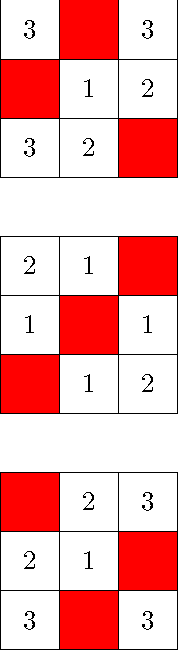
\includegraphics[width=0.2\textwidth]{figures/A/3x3x3_numbered_heatmap.pdf}
%\caption{}
%\label{fig:3x3x3_numbered_heatmap}
%\end{figure}

% (6,4,3)
\begin{con}
\label{con:6x4x3}
The grid $G(6,4,3)$ is perfect.
\end{con}

\begin{proof}
See Figure \ref{fig:4x6x3_numbered_heatmap}.
\end{proof}

\begin{figure}[H]
\centering
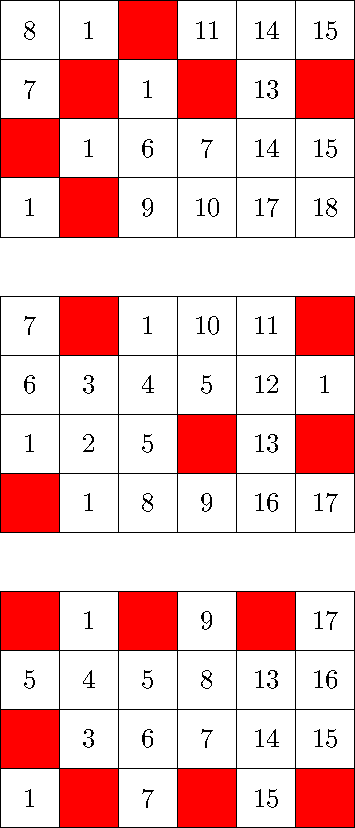
\includegraphics[width=0.25\textwidth]{figures/A/4x6x3_numbered_heatmap.pdf}
\caption{Time-steps of infection from a perfect lethal set on $G(6,4,3)$.}
\label{fig:4x6x3_numbered_heatmap}
\end{figure}

\newpage

% (5, 5, 5)
%\begin{con}
%\label{con:5x5x5}
%The grid $(5,5,5)$ is perfect.
%\end{con}

%\begin{proof}
%See Figure \ref{fig:5x5x5_numbered_heatmap}.
%\end{proof}

%\begin{figure}[H]
%\centering
%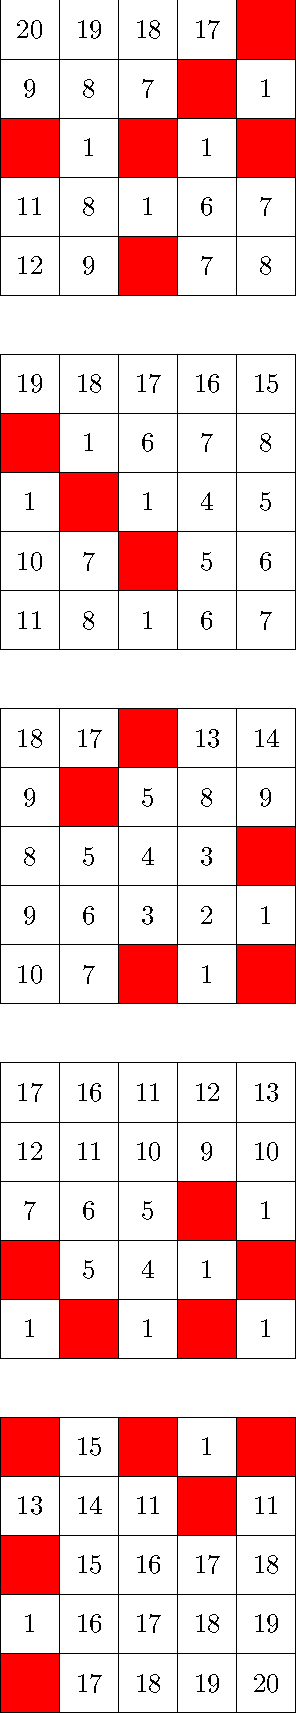
\includegraphics[width=0.2\textwidth]{figures/7/5x5x5_numbered_heatmap.pdf}
%\caption{}
%\label{fig:5x5x5_numbered_heatmap}
%\end{figure}

% (8, 5, 5)
\begin{con}
\label{con:8x5x5}
The grid $G(8,5,5)$ is perfect.
\end{con}

\begin{proof}
See Figure \ref{fig:5x8x5_numbered_heatmap}.
\end{proof}

\begin{figure}[H]
\centering
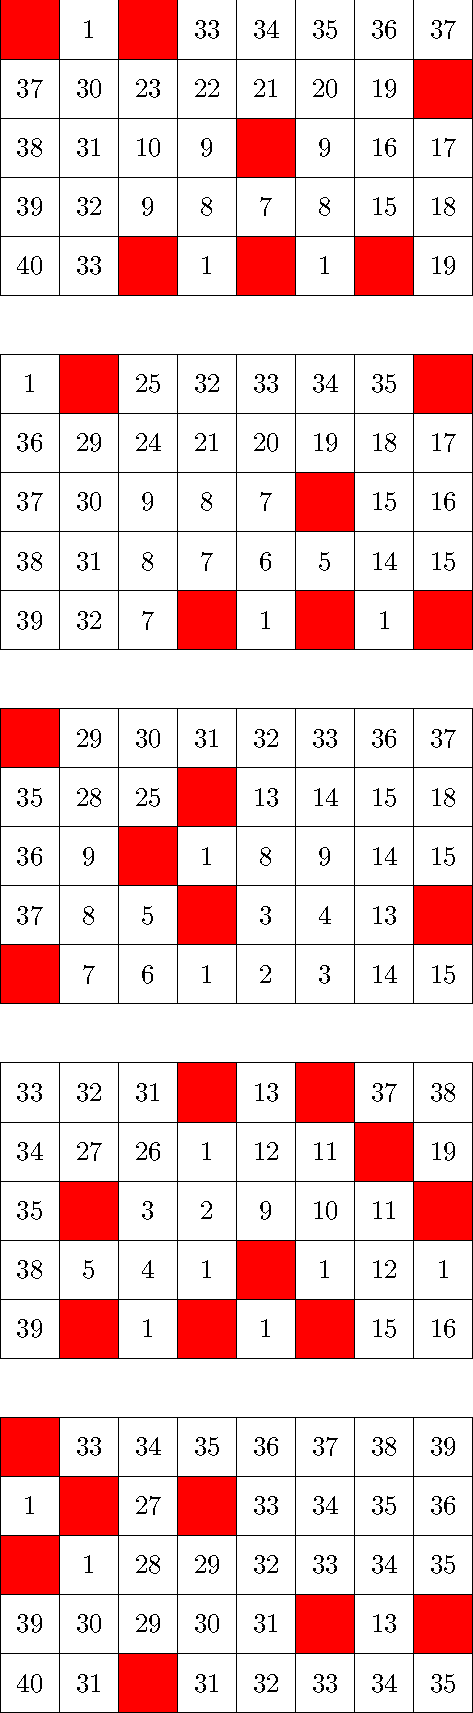
\includegraphics[width=0.35\textwidth]{figures/7/5x8x5_numbered_heatmap.pdf}
\caption{Time-steps of infection from a perfect lethal set on $G(8,5,5)$.}
\label{fig:5x8x5_numbered_heatmap}
\end{figure}

\newpage

% (9, 6, 5)
\begin{con}
\label{con:9x6x5}
The grid $G(9,6,5)$ is perfect.
\end{con}

\begin{proof}
See Figure \ref{fig:6x9x5_numbered_heatmap}.
\end{proof}

\begin{figure}[H]
\centering
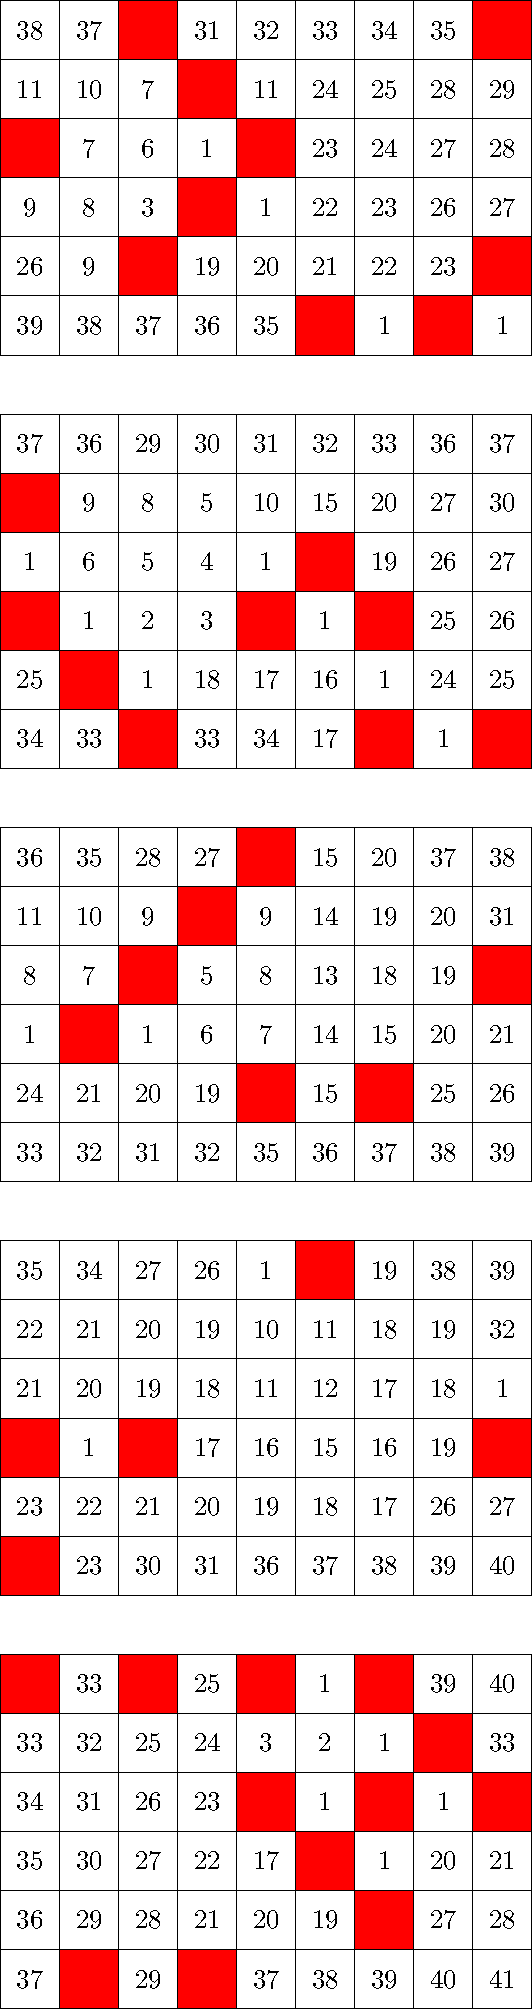
\includegraphics[width=0.33\textwidth]{figures/A/6x9x5_numbered_heatmap.pdf}
\caption{Time-steps of infection from a perfect lethal set on $G(9,6,5)$.}
\label{fig:6x9x5_numbered_heatmap}
\end{figure}

\newpage

% (0 mod 6, 3 mod 6, 2)

\begin{figure}[H]
\centering
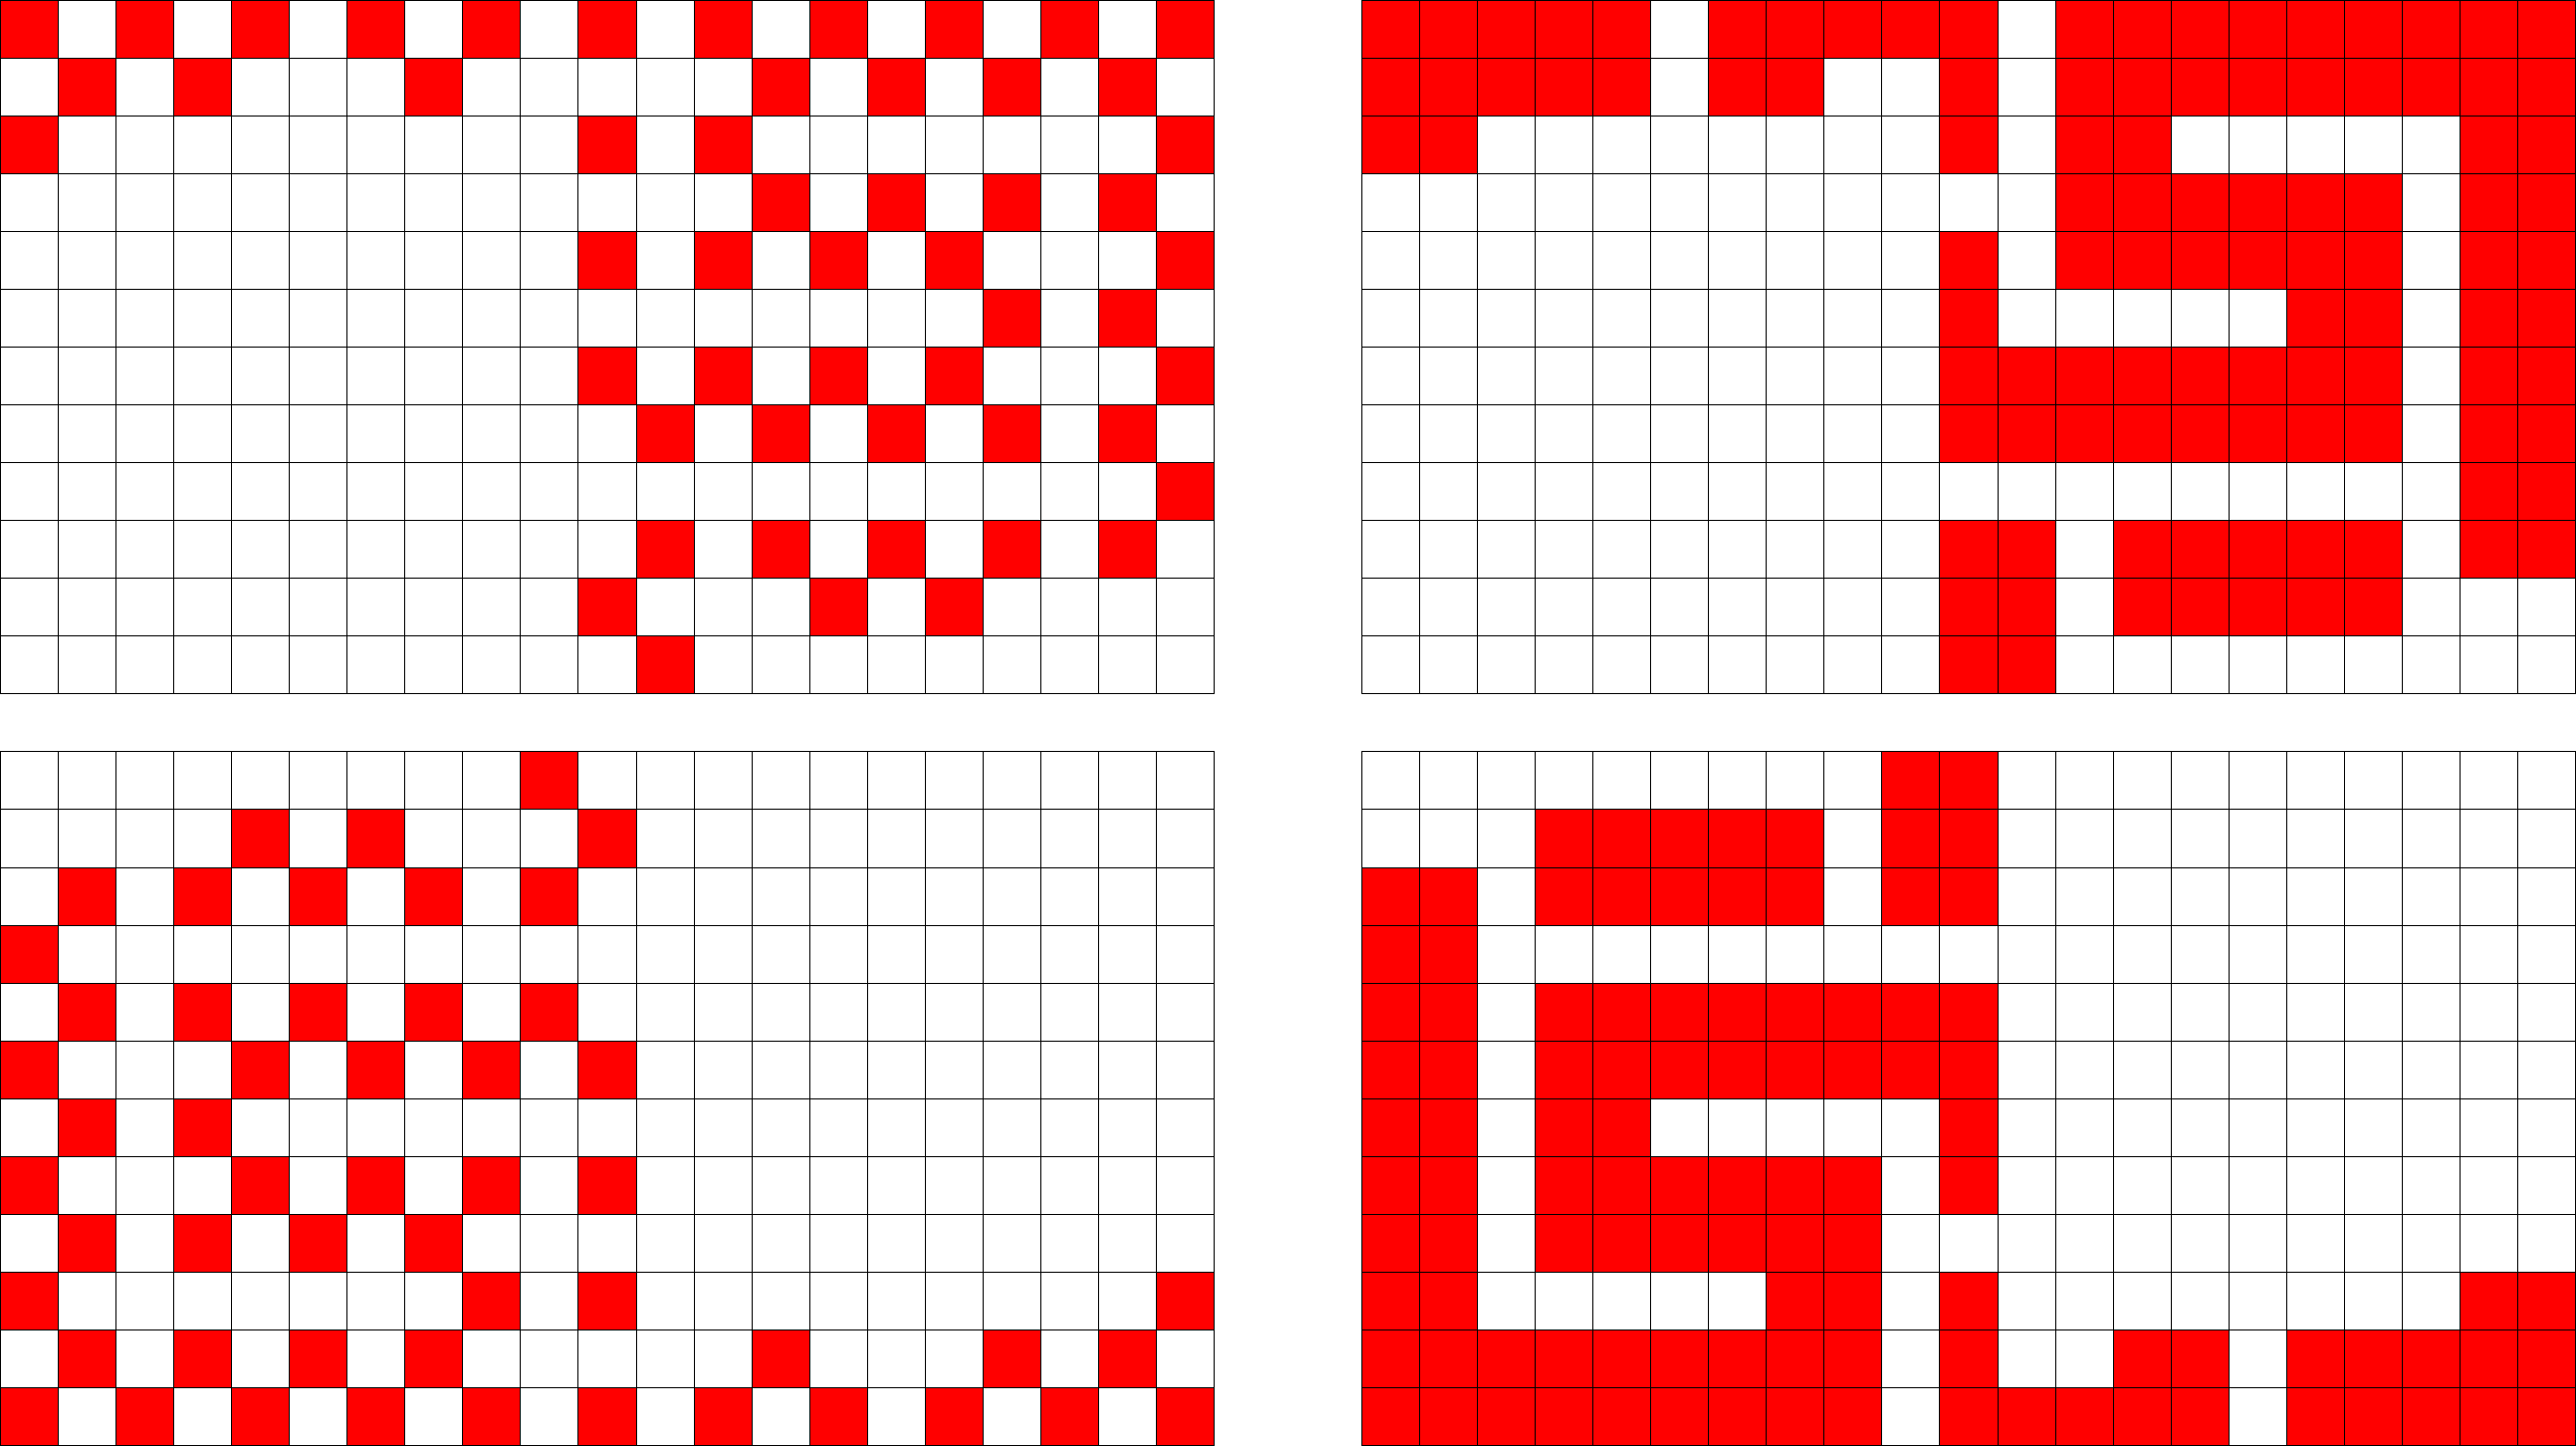
\includegraphics[width=0.8\textwidth]{figures/7/12x21x2.pdf}
\caption{A perfect percolating set for $G(12,21,2)$.}
\label{fig:12x21x2}
\end{figure} 

\begin{figure}[H]
\centering
\begin{subfigure}{0.45\textwidth}
	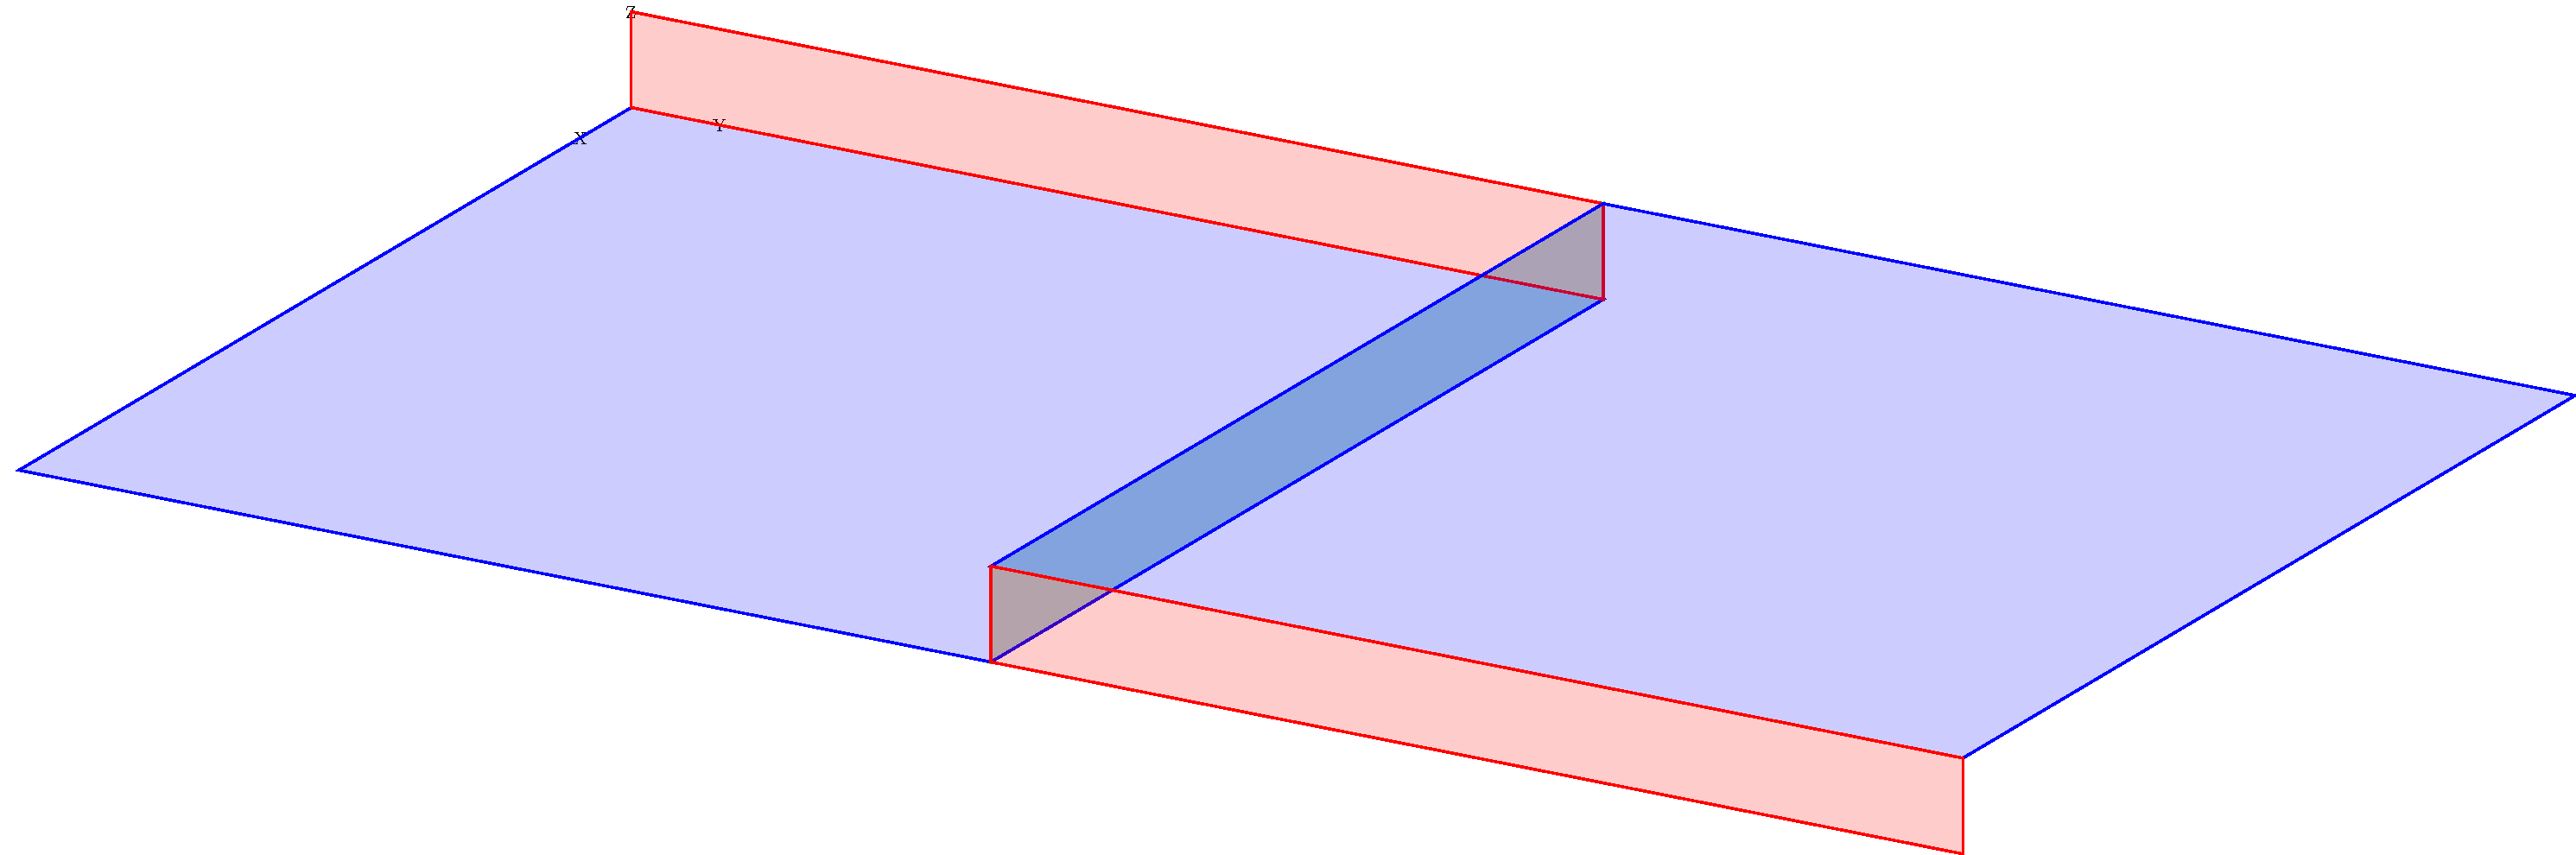
\includegraphics[width=\textwidth]{figures/7/12x21x2_manifold_3d.pdf}
	\caption{A manifold of $G= (12,21,2)$.}
	\label{}
\end{subfigure} \hfill%
\begin{subfigure}{0.45\textwidth}
	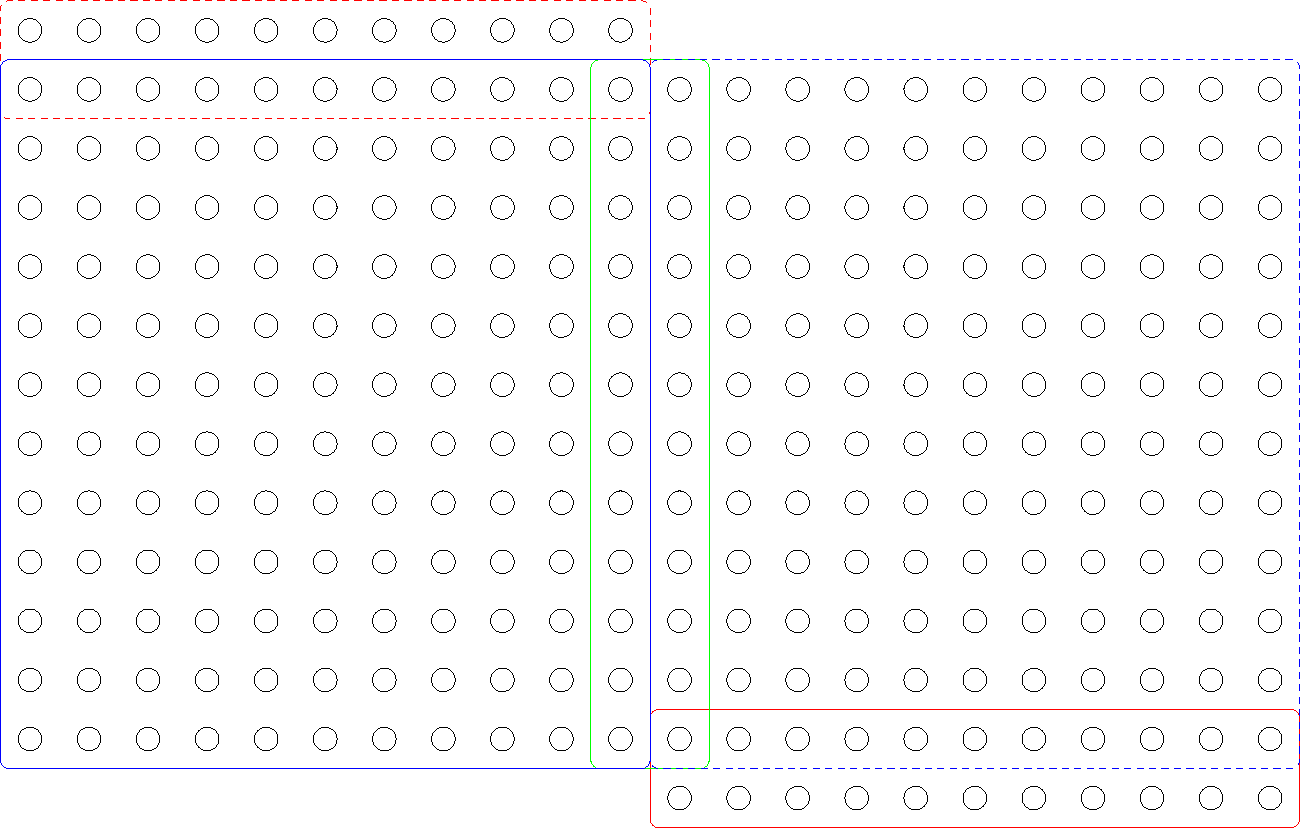
\includegraphics[width=\textwidth]{figures/7/12x21x2_unfolded.pdf}
	\caption{A proper unfolding of $G$.}
	\label{}
\end{subfigure}
\caption{A proper unfolding of $G=G(12,21,2)$. Colored rectangles indicate planes of $G$. Dashed lines indicate that cells appear on different layers. }
\label{fig:12x21x2_unfolded}
\end{figure} 

\begin{figure}[H]
\centering
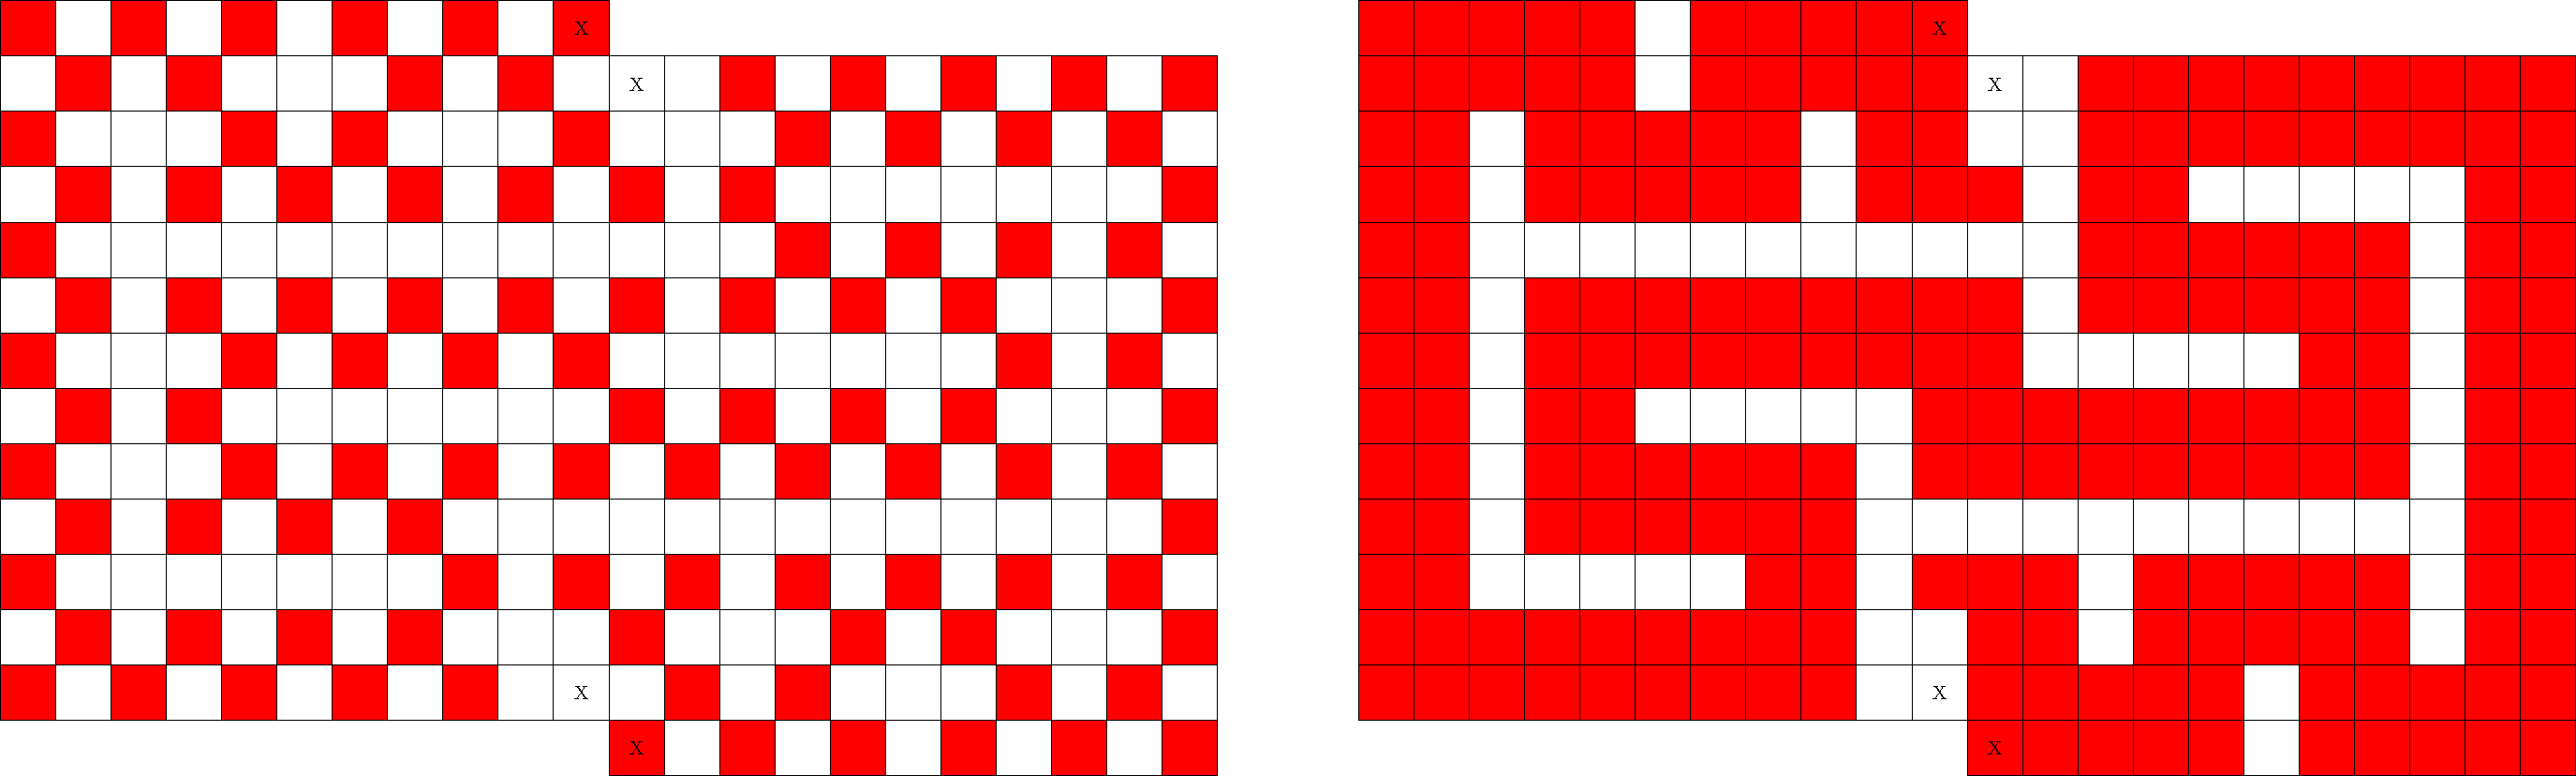
\includegraphics[width=0.8\textwidth]{figures/7/12x21x2_unfolded_lethal.pdf}
\caption{A percolating set on the proper unfolding of $G(12,21,2)$.}
\label{fig:12x21x2_unfolded_lethal}
\end{figure} 

\newpage

\section{Optimal constructions}

% (6,5,5)
\begin{con}
\label{con:6x5x5}
The grid $G(6,5,5)$ is optimal.
\end{con}

\begin{proof}
See Figure \ref{fig:6x5x5_numbered_heatmap}.
\end{proof}

\begin{figure}[H]
\centering
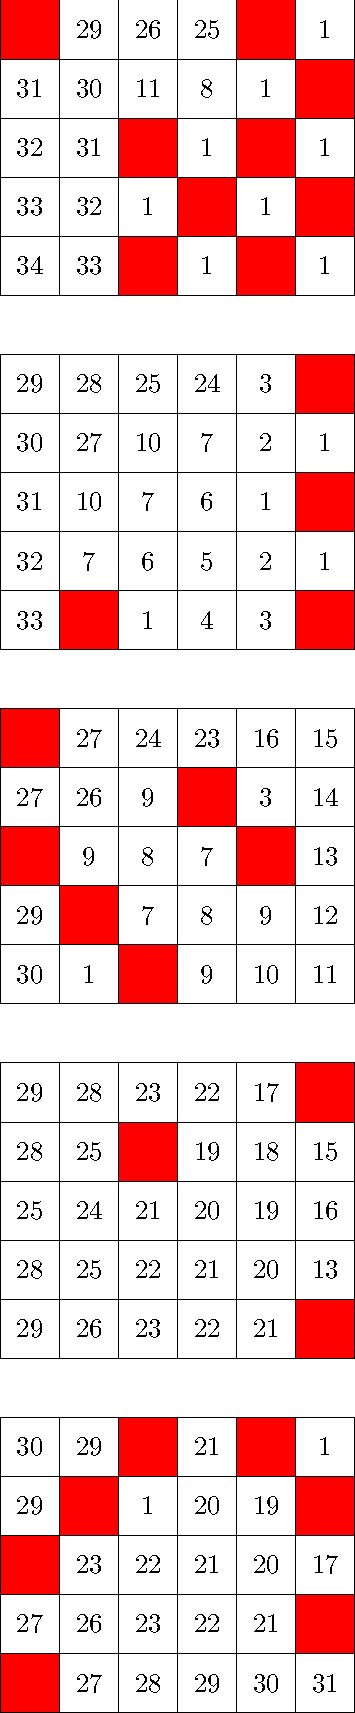
\includegraphics[width=0.24\textwidth]{figures/A/6x5x5_numbered_heatmap.pdf}
\caption{Time-steps of infection from an optimal lethal set on $G(6,5,5)$.}
\label{fig:6x5x5_numbered_heatmap}
\end{figure}

\newpage

% (7,5,5)
\begin{con}
\label{con:7x5x5}
The grid $G(7,5,5)$ is optimal.
\end{con}

\begin{proof}
See Figure \ref{fig:7x5x5_numbered_heatmap}.
\end{proof}

\begin{figure}[H]
\centering
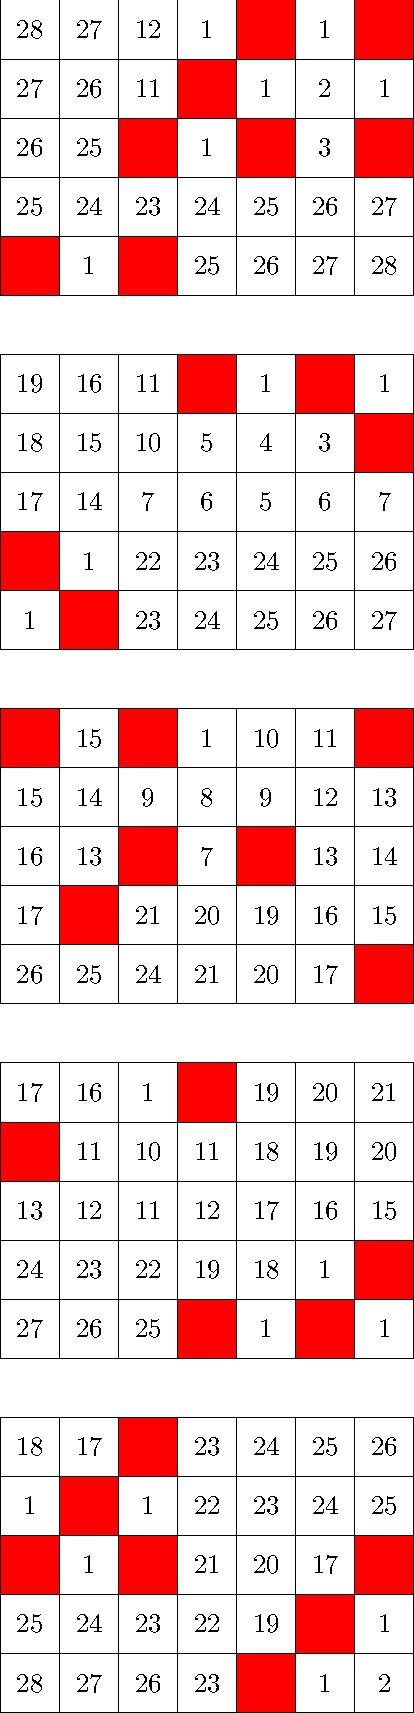
\includegraphics[width=0.3\textwidth]{figures/A/7x5x5_numbered_heatmap.pdf}
\caption{Time-steps of infection from an optimal lethal set on $G(3,3,1)$.}
\label{fig:7x5x5_numbered_heatmap}
\end{figure}

\newpage

% (7,6,5)
\begin{con}
\label{con:7x6x5}
The grid $G(7,6,5)$ is optimal.
\end{con}

\begin{proof}
See Figure \ref{fig:7x6x5_numbered_heatmap}.
\end{proof}

\begin{figure}[H]
\centering
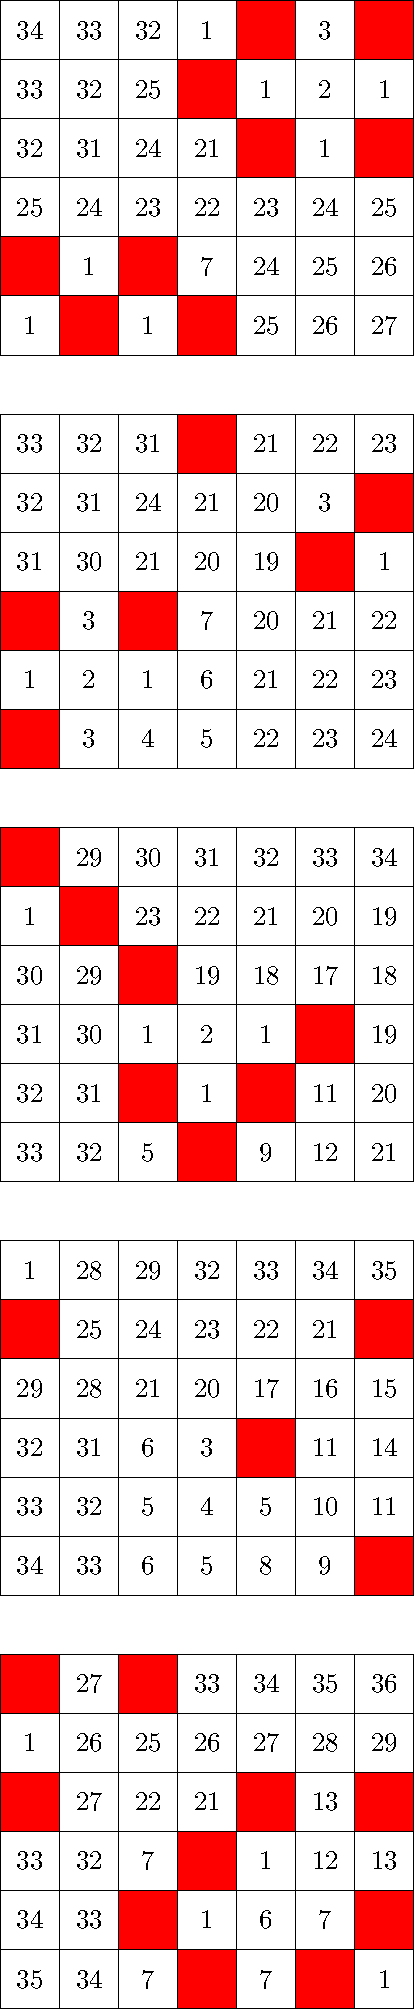
\includegraphics[width=0.26\textwidth]{figures/A/7x6x5_numbered_heatmap.pdf}
\caption{Time-steps of infection from an optimal lethal set on $G(7,6,5)$.}
\label{fig:7x6x5_numbered_heatmap}
\end{figure}

\newpage

% (7,7,5)
\begin{con}
\label{con:7x7x5}
The grid $G(7,7,5)$ is optimal.
\end{con}

\begin{proof}
See Figure \ref{fig:7x7x5_numbered_heatmap}.
\end{proof}

\begin{figure}[H]
\centering
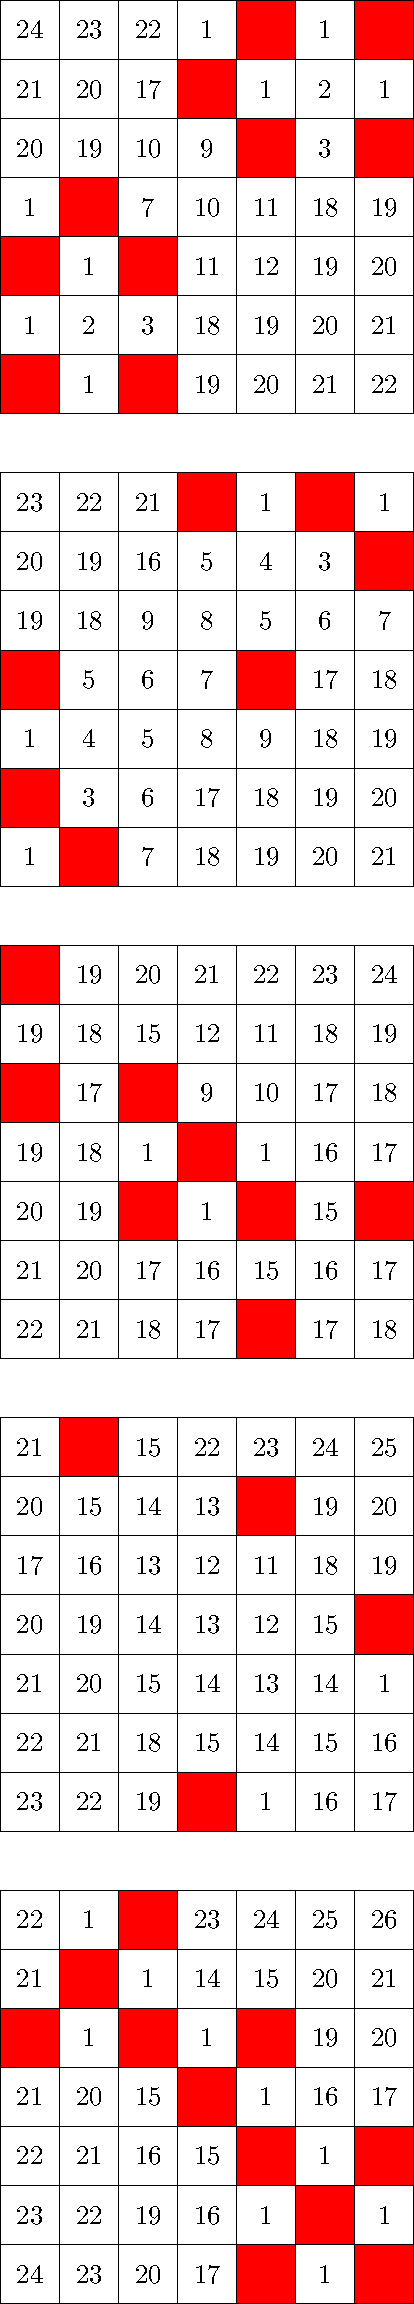
\includegraphics[width=0.23\textwidth]{figures/A/7x7x5_numbered_heatmap.pdf}
\caption{Time-steps of infection from an optimal lethal set on $G(7,7,5)$.}
\label{fig:7x7x5_numbered_heatmap}
\end{figure}


